\section*{Цель работы}

Целью работы является реализация программы для генерации псевдослучайных чисел
с использованием табличного и алгоритмического методов. Также необходимо
выбрать метрику для оценки случайности последовательности чисел и вычислить ее
значение для сгенерированного набора.

\section*{Алгоритмы генерации псевдослучайных чисел}

На практике применяют три основных способа генерации случайных чисел:
\begin{itemize}
    \item аппаратный --- случайная величина вырабатывается специальной
          электрической приставкой (генератор случайных чисел) как правило
          внешнее устройство компьютера не требует других устройств и операций
          кроме обращения к устройству;
    \item табличный --- случайные числа оформляются в виде таблицы;
    \item алгоритмический --- применяются специализированные алгоритмы.
\end{itemize}

\begin{threeparttable}
\caption{Сравнение методов генерации псевдослучайных чисел}
\centering
\small
\begin{tabular}{|l|l|l|}
\hline
Способ                           & Достоинства                                                                               & Недостатки                                                                             \\ \hline
\multirow{4}{*}{Аппаратный}      & Запас чисел неограничен                                                                   & \begin{tabular}[c]{@{}l@{}}Неустойчивость к внешнему\\ воздействию\end{tabular}        \\ \cline{2-3} 
                                 & \begin{tabular}[c]{@{}l@{}}Мало вычислительных\\ операций\end{tabular}                    & \begin{tabular}[c]{@{}l@{}}Нельзя воспроизвести\\ последовательность\end{tabular}      \\ \cline{2-3} 
                                 & \begin{tabular}[c]{@{}l@{}}Не занимает место\\ в памяти\end{tabular}                      & \begin{tabular}[c]{@{}l@{}}Используются специальные\\ устройства\end{tabular}          \\ \cline{2-3} 
                                 &                                                                                           & \begin{tabular}[c]{@{}l@{}}Необходимы меры\\ стабилизации\end{tabular}                 \\ \hline
\multirow{3}{*}{Табличный}       & \begin{tabular}[c]{@{}l@{}}Можно воспроизвести\\ последовательность\end{tabular}          & Запас чисел ограничен                                                                  \\ \cline{2-3} 
                                 & \begin{tabular}[c]{@{}l@{}}Однократная проверка\\ на случайность\end{tabular}             & \begin{tabular}[c]{@{}l@{}}Занимает место в памяти\\ и на диске\end{tabular}           \\ \cline{2-3} 
                                 &                                                                                           & Затраты на обращение к памяти                                                          \\ \hline
\multirow{4}{*}{Алгоритмический} & \begin{tabular}[c]{@{}l@{}}Однократная проверка\\ на случайность\end{tabular}             & Запас чисел ограничен периодом                                                         \\ \cline{2-3} 
                                 & \begin{tabular}[c]{@{}l@{}}Многократное воспроизведение\\ последовательности\end{tabular} & \begin{tabular}[c]{@{}l@{}}Существенные затраты\\ вычислительных ресурсов\end{tabular} \\ \cline{2-3} 
                                 & Малые затраты памяти                                                                      &                                                                                        \\ \cline{2-3} 
                                 & \begin{tabular}[c]{@{}l@{}}Не требуются специальные\\ устройства\end{tabular}             &                                                                                        \\ \hline
\end{tabular}
\end{threeparttable}

\section*{Линейный конгруэнтный метод}

В качестве алгоритмического метода генерации псевдослучайных чисел был выбран
линейный конгруэнтный метод. Для осуществления генерации чисел данным методом,
необходимо задать 4 числа:
\begin{itemize}
    \item $m > 0$ --- модуль;
    \item $0 \leq a	\leq m$ --- множитель;
    \item $0 \leq c \leq m$ --- приращение;
    \item $0 \leq X_0 \leq m$ --- начальное значение.
\end{itemize}

Последовательность случайных чисел генерируется при помощи следующего
рекуррентного соотношения:
\begin{equation*}
    X_{n+1} = (a X_n + c) \mod m
\end{equation*}

В качестве значений коэффициентов были выбраны соответствующие значения
для реализации функции \code{rand} из \code{glibc}:
\begin{align*}
    m & = 2 ^ {32} \\
    a & = 1103515245 \\
    c & = 12345.
\end{align*}

\section*{Табличный метод}

Табличный метод базируется на выборке и методе, описанных в\\ГОСТ 11.003-73

Генерация случайных числе производится на основании 8 таблиц, содержащих 1024
цифры.

Выбор случайного последовательности из $n$ $l$-разрядных чисел в диапазоне
$[a, b]$ выполняется по следующим правилам:
\begin{itemize}
    \item используя начальное смещение выбирается таблица, строка
          и столбец;
    \item относительно начальной позиции выбираются $n \cdot l$ цифр при
          движении слева направо, сверху вниз; если текущая таблица содержит
          меньшее требуемого количество цифр, то необходимо перейти к следующей
          таблице; в случае исчерпания последней таблицы, указатель переходит
          в начало первой таблицы;
    \item выбранные цифры объединяются в группы по $l$ элементов, что
          является представлением $l$-разрядного числа;
    \item если число не подходит под указанный диапазон, оно --- вычеркивается,
          и из таблицы выбирается следующее число.
\end{itemize}

\section*{Критерий проверки $\chi^2$}

Критерий $\chi^2$ является критерием проверки простой непараметрической
гипотезы о законе распределения дискретной случайной величины $X$.

Пусть $X$ может принимать $l$ различных значений $a_1, \dots, a_l$ с
вероятностями $p_1, \dots, p_l$ соответственно ($\frac{1}{l}$ в случае
равномерного распределения).

Тогда, если $X_n$ --- случайная выборка размера $n$, то для определения
ее случайности может использоваться следующую статистику
\begin{equation*}
    \Delta(\overrightarrow{X_n}) = \sum_{i = 1}^{l} \frac{(n_i(\overrightarrow{X_n}) - n p_i) ^ 2}{n p_i},
\end{equation*}
где $n_i(\overrightarrow{X_n})$ --- случайная величина, принимающая для каждой
реализации $\overrightarrow{x_n}$ случайной выборки $\overrightarrow{X_n}$
значение, равное числу компонент выборки, имеющих значение $a_i$.
Малые значения данной статистики связаны с близостью фактических
значений вероятности появления числа в последовательности с теоретическим
значением $\frac{1}{l}$.

Доказано, что статистика $\Delta(\overrightarrow{X_n})$ слабо сходится
к случайной величине, имеющей распределение $\chi^2$ с $l - 1$ степенями
свободы, при $n \rightarrow \infty$.

Таким образом, значение $1 - \chi^2_{l - 1}(\Delta(\overrightarrow{x_n}))$,
где $\chi^2_{l - 1}(\Delta(\overrightarrow{x_n}))$ --- значение функции
распределения $\chi^2$ для значения $\Delta(\overrightarrow{x_n})$, может
быть использовано для оценки случайности последовательности, чем
ближе значение метрики к 1, тем более случайна выборка, и наоборот, если
значение близко к 0, то выборка --- неслучайна.

Так как проверяется гипотеза о равномерности закона распределения генератора,
то значение статистики может быть вычислено следующим образом
\begin{equation*}
    \Delta(\overrightarrow{X_n}) = \frac{l}{n} \sum_{i = 1}^{l} n_i(\overrightarrow{X_n}) ^ 2 - n,
\end{equation*}

\section*{Текст программы}
\begin{lstlisting}[caption={Интерфейс генератора случайных чисел}, language=python]
from abc import ABC, abstractmethod

class RandomChecker(ABC):
    @abstractmethod
    def check(self, sequence: list[int]) -> float:
        pass

class Randomizer(ABC):
    @abstractmethod
    def get(self) -> int:
        pass

class RandomizerCreator(ABC):
    @abstractmethod
    def create(self, a: int, b: int) -> Randomizer:
        pass
\end{lstlisting}

\begin{lstlisting}[caption={Класс, реализующий линейный конгруэнтный метод}, language=python]
from time import time

from src.randomizer import Randomizer, RandomizerCreator

class LinearCongruentRandomizer(Randomizer):
    def __init__(self, a: int, c: int, m: int, i: int,
                 min: int, max: int):
        self.a = a
        self.c = c
        self.m = m

        self.current = i % self.m

        self.min = min
        self.rng = max - min + 1

    def get(self) -> int:
        self.current = (self.a * self.current + self.c) \
                       % self.m

        return self.min \
               + int(round(self.rng * (self.current
                                       / (self.m - 1))
                           - 0.5,
                           0))

class LinearCongruentRandomCreator(RandomizerCreator):
    def __init__(self, a: int, c: int, m: int):
        self.a = a
        self.c = c
        self.m = m

    def create(self, a: int, b: int) -> Randomizer:
        return LinearCongruentRandomizer(self.a, self.c,
                                         self.m,
                                         int(time() * 1e6),
                                         a, b)
\end{lstlisting}

\begin{lstlisting}[caption={Класс, реализующий табличный метод}, language=python]
from time import time
from math import log10

from src.randomizer import Randomizer, RandomizerCreator

class TableRandomizer(Randomizer):
    def __init__(self, values: list[int], seed: int,
                 min: int, max: int):
        self.values = values
        self.current = seed % len(self.values)
        self.min = min
        self.max = max
        self.l = int(log10(self.max)) + 1
        self.limit = len(self.values)

    def get(self) -> int:
        num = self.min - 1

        while self.min > num or self.max < num:
            num = self.values[self.current]
            self.current = (self.current + 1) % self.limit

            for _ in range(self.l - 1):
                num = num * 10 + self.values[self.current]
                self.current = (self.current + 1) \
                               % self.limit

        return num

class TableRandomCreator(RandomizerCreator):
    def __init__(self, filename: str):
        file = open(filename, "r")
        content = file.read()
        file.close()
        self.values = list(map(lambda x: int(x),
                               content[:-1]))

    def create(self, a: int, b: int) -> Randomizer:
        return TableRandomizer(self.values,
                               int(time() * 1e6), a, b)
\end{lstlisting}

\begin{lstlisting}[caption={Класс, реализующий критерий $\chi^2$}, language=python]
from scipy.stats import chi2

from src.randomizer import RandomChecker

class Chi2RandomChecker(RandomChecker):
    def check(self, sequence: list[int]) -> float:
        values = {}
        n = len(sequence)
        range = max(sequence) - min(sequence) + 1

        for i in sequence:
            if i in values:
                values[i] += 1
            else:
                values[i] = 1

        sum_sqr = sum(map(lambda x : values[x] * values[x],
                          values))
        val = range / n * sum_sqr - n

        return 1 - chi2.cdf(val, range - 1)
\end{lstlisting}

\section*{Результаты работы}

\begin{figure}[h]
    \begin{minipage}{0.3\textwidth}
        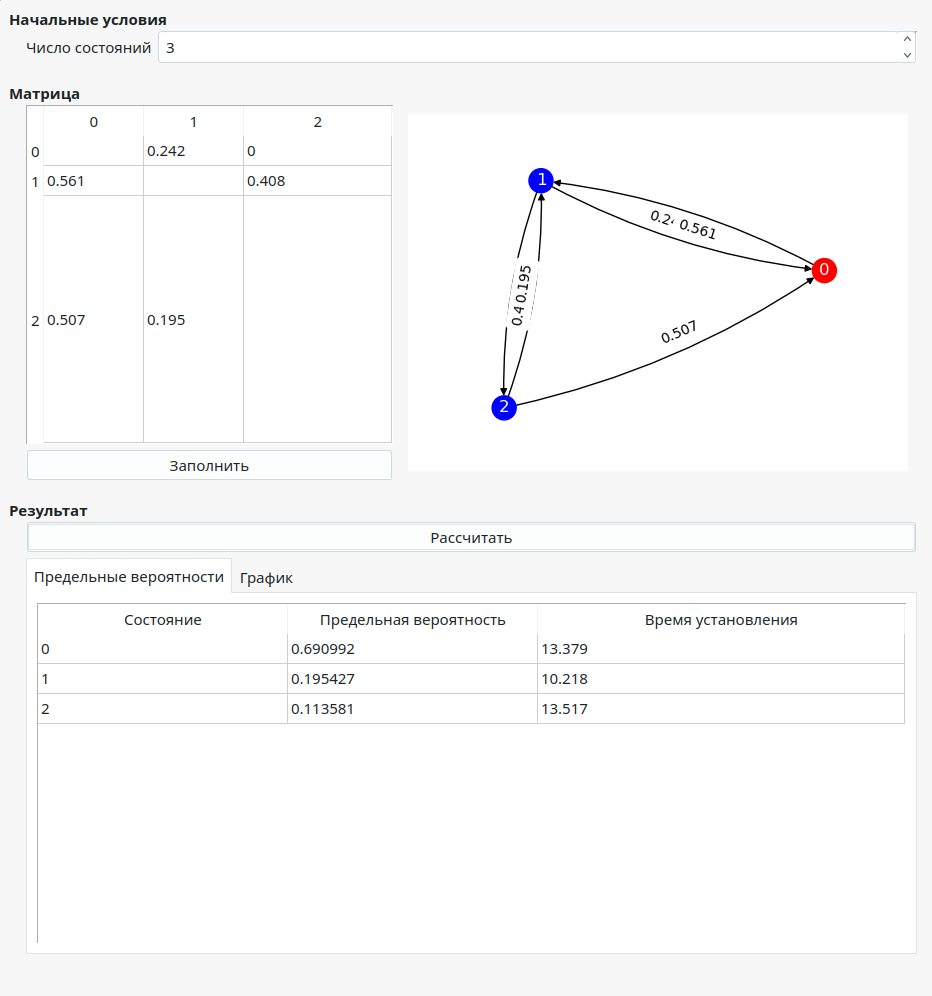
\includegraphics[width=\linewidth]{1.png}
    \end{minipage}
    \hfill
    \begin{minipage}{0.3\textwidth}
        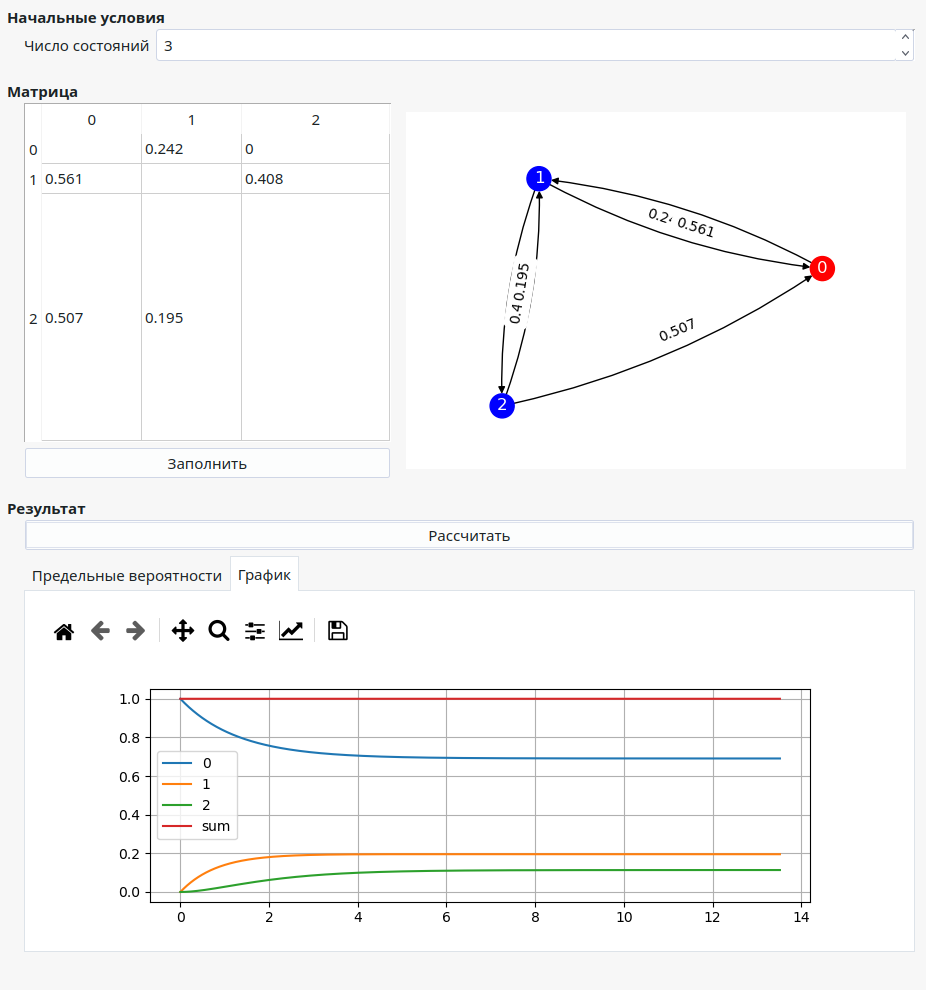
\includegraphics[width=\linewidth]{2.png}
    \end{minipage}
    \hfill
    \begin{minipage}{0.3\textwidth}
        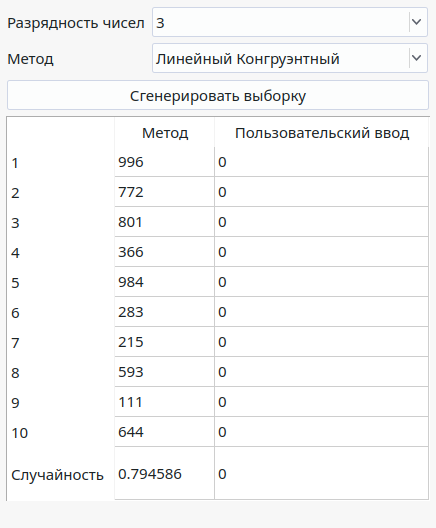
\includegraphics[width=\linewidth]{3.png}
    \end{minipage}
    \caption{Результаты работы программы для линейного конгруэнтного метода}
\end{figure}

\begin{figure}[h]
    \begin{minipage}{0.3\textwidth}
        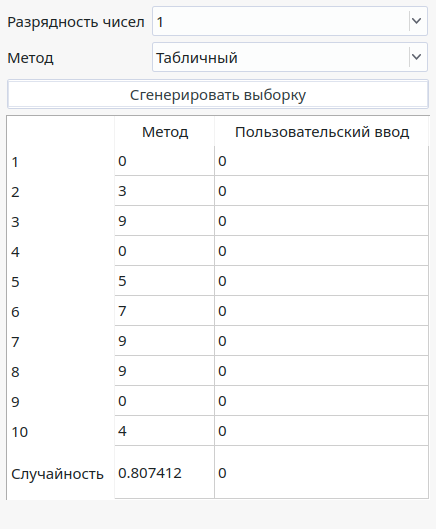
\includegraphics[width=\linewidth]{4.png}
    \end{minipage}
    \hfill
    \begin{minipage}{0.3\textwidth}
        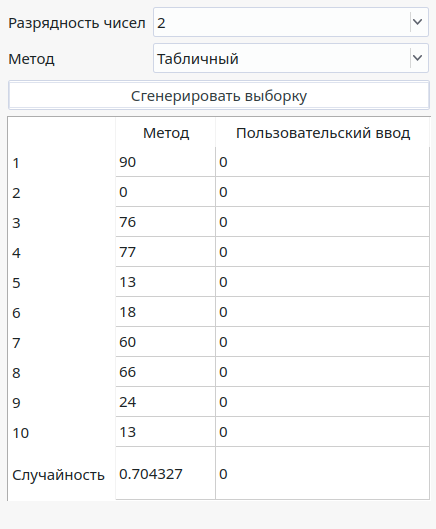
\includegraphics[width=\linewidth]{5.png}
    \end{minipage}
    \hfill
    \begin{minipage}{0.3\textwidth}
        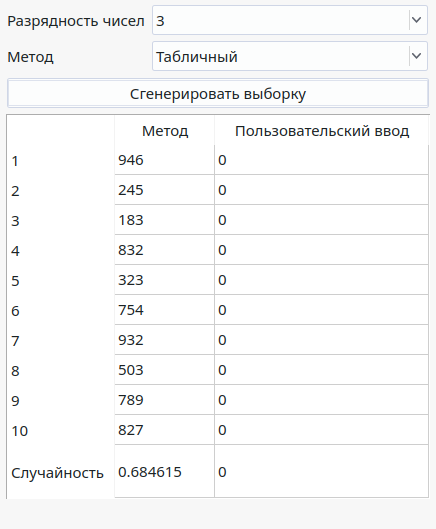
\includegraphics[width=\linewidth]{6.png}
    \end{minipage}
    \caption{Результаты работы программы для табличного метода}
\end{figure}

\clearpage

\section*{Вывод}

В ходе выполнения лабораторной работы была разработана программа для генерации
псевдослучайных чисел с использованием табличного и линейного конгруэнтного
методов. Также была реализована возможность оценки случайности
последовательности чисел с использованием критерия $\chi^2$.

